% vim: spelllang=de
\documentclass[a5paper,ngerman,9pt]{article}
\usepackage[T1]{fontenc}
\usepackage[utf8]{inputenc}
\usepackage[margin=0.5in,includefoot]{geometry}
\usepackage{microtype}
\usepackage{babel}
\usepackage[none]{solarized}
\usepackage{sectsty}
\usepackage{ccfonts}
\usepackage{euler}
\usepackage{jscript}
\usepackage{html}
\usepackage{todone}
\usepackage{fancyhdr}
\usepackage{fancyvrb}
\usepackage{graphicx}
\usepackage{multicol}
\pagestyle{fancy}
\fancypagestyle{plain}{
\fancyhf{}
\fancyfoot[C]{{\color{deemph}\small$\thepage$}}
\renewcommand{\headrulewidth}{0pt}
\renewcommand{\footrulewidth}{0pt}}
\title{\color{emph}Programmieren Lernen}
\author{Timm Knape}
\date{\today}
\columnseprule.2pt
\renewcommand{\columnseprulecolor}{\color{deemph}}
\begin{document}
\pagecolor{background}
\color{normal}
\allsectionsfont{\color{emph}\mdseries}
\pagestyle{plain}
\maketitle
\thispagestyle{fancy}
\surroundwithmdframed[backgroundcolor=codebackground,fontcolor=normal,hidealllines=true]{Verbatim}


\section{Programmieren ist Zauberei}

\begin{multicols}{2}
	\subsection{Im Keller}

	Das Gewölbe ist düster.
	Grauer Rauch steigt langsam wabernd aus großen, bronzenen Schalen
	auf.
	Von unsichtbaren LED-Strahlern wird er lila angestrahlt und
	mystifiziert die gesamte Szene.
	Leise klirren indische Klang-Schalen kreuz und quer, ohne sich
	verorten zu lassen.

	Ein Mann in langem Mantel steht auf einmal mitten im Raum.
	Niemand hat ihn kommen sehen.
	Auf dem Mantel sind mit goldenen Fäden Symbole aus unterschiedlichen
	Schrift-Systemen aufgestickt.
	Wenn etwas nach einem bekannten lateinischen Buchstaben aussieht,
	dann ist es sicherlich ein griechisches, kyrillisches oder ganz
	anderes Symbol.

	Der Mann breitet langsam die Arme aus.
	Gleichzeitig verändert sich der Raum.
	Die Temperatur sinkt.
	Das Licht nimmt sich zurück.
	Nur eine gelbe Lichtsäule bildet sich um den Magier.

	Wo vorher noch unbestimmte Leere war, leuchtet nun ein Pentagramm
	auf dem groben Felsboden.
	In dessen Mitte steht der Zauberkundige.

	Er murmelt kaum verständlich eine Beschwörungsformel in einer
	fremden Sprache.
	Teile erinnern an Latein.
	Dabei bewegen sich seine Finger als wären sie zu einem eigenen,
	unabhängigen Leben erwacht und erkunden wie frisch geschlüpfte
	Küken die große Welt.

	Ruckartig senkt er die Arme.
	Ein Donnerschlag dröhnt durch die Halle.
	Ein kleiner Bistro-Tisch steht wie aus dem Nichts vor ihm.
	Auf diesem liegen dampfende Papp-Kartons.

	„Bitte nehmen Sie sich, Ihre Pizza. Ich hoffe, der Tag hat Ihnen
	gefallen.“

	Mit einer knappen Verbeugung verabschiedet sich der Künstler und
	verläßt das Gewölbe, in dem eine Management-Schulung zu ihrem
	Abschluß gekommen ist.

	\subsection{Quer-Bezug}

	Ja und?
	Was hat das alles mit Programmieren zu tun?
	Eine Menge!

	Für den Außenstehenden wirkt Programmieren wie Magie.
	Programmierkundige können seelenlose Maschinen zum Leben erwecken.
	Durch die zunehmende Vernetzung werden die Programme scheinbar
	allwissend.

	Wie ein böser Dämon müssen sie von ihrem Meister bebändigt und in
	Zaum gehalten werden.

	Aber gleichzeitig ist das Programmieren für erfahrene Programmierer
	eben keine Hexerei.
	So wie auch ein Zauberkünstler keine echte Magie braucht, um seine
	Kunststücke vorzuführen.

	Dieses Buch ist der erste Schritt einer Anleitung zum Programmieren.
	
	Alles was du brauchst ist ein Gerät mit Internet-Anschluß, auf dem
	ein Web-Browser läuft.
	Zum Beispiel ein Tablet oder Smart-Phone.
	Oder ein Laptop.
	Oder ein Desktop-Computer.
	Das sind diese Kisten mit abgesetzten Bildschirm und Tastatur.

	Damit können wir ein klein wenig programmieren lernen.
	Es ist gar nicht so schwer.
	Die Programme sind unsere Zaubersprüche.
	Der Web-Browser ist der Raum, in dem wir wirken.
	Und mit etwas Geduld entstehen komplexe Gebilde, die scheinbar
	viel mächtiger sind, als die paar Zeilen Programm-Text vermuten
	lassen.

	Lass uns das Spiel beginnen!
\end{multicols}

\section{Um was geht es?}

\begin{multicols}{2}
	\subsection{Definitionen}

	Es ist total wichtig, dass wir ganz klar Wissen, um was es überhaupt
	geht.
	Wenn wir kein gemeinsames Verständnis der verwendeten Begriffe haben,
	dann ist es höchstens Glück, wenn Wissen und Erkenntnis transportiert
	werden.
	Das kann funktionieren. Muss es aber nicht.

	Zuerst geht es um unsere eigene Rolle.
	Der \emph{Programmierer} oder die \emph{Programmiererin} erstellen
	Programme.
	Gute Programmierer zeichnen sich dadurch aus, dass sie recht schnell
	Programme erstellen können, die relativ wenig Fehler haben und
	selber schnell laufen.
	Aber das sind vorerst nur Details.
	Wichtig ist: Wir müssen Programme schreiben.

	\emph{Programme} selbst sind Anweisungen, die so klar und haarklein
	umrissen sind, dass selbst ein Computer sie ausführen kann.
	Es gibt unterschiedliche \emph{Programmiersprachen}, in denen
	Programme formuliert werden können.

	Ein Beispiel ist JavaScript, das heute in fast jedem Web-Browser
	verwendet werden kann.
	Aber JavaScript hat so seine Tücken.
	Es wird leichter sein, mit einer einfacheren Sprache anzufangen.

	Als drittes Element gibt es noch die \emph{Maschine}, welche ein
	Programm ausführt.
	Das kann ein Computer sein.
	Muss es aber nicht.

	Das folgenden Beispiel zeigt, wie man schon um 1900 ein Programm
	ganz ohne Elektronik schreiben und ausführen konnte.

	\subsection{Beispiel: Taylorismus}

	Die Fabriken sind ein schönes Beispiel für das nicht-elektronische
	Ausführen eines Programms.
	Man spricht auch gerne vom Abarbeiten eines Programms:
	Es gibt eine Liste von Schritten, die nacheinander ausgeführt werden
	müssen.

	Zur Ehre des großen Pionier-Geists von Henry Ford und der Besinnung
	als Teil einer Auto-Nation, habe ich ein etwas vereinfachtes
	Programm geschrieben, wie ein Auto in einer Fabrik gebaut wird:

	\begin{enumerate}
		\item Nehme vier Reifen $r_1,\ldots,r_4$.
		\item Nehme ein Lenkrad $rr$.
		\item Baue in wenigen, nicht näher beschriebenen Schritten aus
			$r_1,\ldots,r_4,rr$ mit zusätzlichem Material einen roten
			VW Polo.
	\end{enumerate}

	Natürlich war die eigentliche Liste in Wolfsburg etwas länger.
	Aber die würde den Rahmen sprengen und rechtliche Streitigkeiten
	heraufbeschwören.

	Bleiben wir bei den drei Schritten.

	Die Programmierer in der Fabrik sind die Ingenieure und
	Wissenschaftler, die alle Schritte zusammentragen, die notwendig
	sind, um ein Auto zu bauen.

	Je genauer die Schritte beschrieben sind, desto einheitlicher sind
	die resultierenden Autos.
	Und desto weniger muss der Fließband-Arbeiter in der Fabrik vom
	Auto-Bauen verstehen.

	In unserem vereinfachten Programm sind die ersten beiden Schritte
	mit einigen Minuten anlernen ausführbar:
	Da hinten liegen Reifen, dort im Regal sind die Lenkräder.
	Nun sieh zu!

	Für den dritten Schritt braucht es etwas mehr Expertise.
	Die ich leider selber nicht besitze.
	Daher muss ich beim Auto-Bauen notgedrungen eine sehr kompetente
	Maschine zum Ausführen meines Programms voraussetzen.

	In diesem Beispiel ist die Fabrik-Halle mit ihren Arbeitern,
	Fließ-Bändern und Lackier-Robotern die Maschine, die das Programm
	„ich baue einen Polo“ ausführen kann.

	Dazu benötigt die Fabrik zusätzliches Material als Eingabe.
	Irgendwo müssen auch die Räder und Lenkräder herkommen.
	Auch Betriebsmittel wie Strom und Geld sind notwendig.
	
	Und sie produziert ein Auto als Ausgabe.
	Diese Begriffe werden wir später noch präzisieren müssen.

	\subsection{Etwas realistischer}

	Ein Programm zum Auto-Bauen ist heute gar nicht mehr so abwegig.

	Heute können Autos vielfältig konfiguriert werden.
	Das erleichtert zum einen den Händlern, sich um das Rückgaberecht
	zu drücken.
	Aber auch die Kunden genießen, dass ihr Auto ganz individuell zu
	ihnen passt und nicht in einem Einheits-Schwarz wie alle anderen
	Autos herumfährt. Obwohl schwarz immer noch eine sehr verbreitete
	Farbe ist.

	Aber die Konfiguration eines Autos ist im Prinzip auch ein Programm.
	Es bekommt nicht jeder Arbeiter in der Fabrik eine Kopie meines
	Bestell-Zettels, aber er bekommt eine Liste mit Schritten, die er
	ausführen muss, um genau mein Auto zu bauen.

	Diese Listen werden nicht händisch erstellt.
	Vielmehr gibt es ein Programm, das aus der Konfiguration (die ja wie
	gesagt auch ein Programm ist) ein anderes Programm macht.
	Solche Programme nennt man \emph{Compiler}.
	Und mit ihnen kann man jede Menge Schabernack anstellen.

	\subsection{Andere Namen}

	Zusammen mit dem Programm wird oft der Begriff \emph{Algorithmus}
	verwendet.
	Ein Algorithmus beschreibt, wie ein Programm funktioniert.
	Er ist meistens nicht in einer Programmier-Sprache geschrieben,
	sondern abstrakt.
	Ein Computer kann einen Algorithmus nicht direkt ausführen.
	Ein Mensch kann es jedoch.
	Also ist ein Algorithmus durchaus ein Programm für die Maschine
	Programmierer.
	Meistens übernimmt es dann der Programmierer den Algorithmus in
	ein Programm einer anderen Programmiersprache zu übersetzen, so dass
	ein Computer ihn ausführen kann.

	Aber für uns macht das erst einmal keinen Unterschied.
	Ein Algorithmus ist ein Programm für eine bestimmte Maschine (uns!).
	Ein Algorithmus hat noch zusätzliche Einschränkungen, die an dieser
	Stelle noch nicht behandelt werden sollen.

	Gerne wird anstatt des Begriffs Programm auch der \emph{Prozess}
	verwendet.
	Besonders wenn die ausführende Maschine Menschen enthält.
	Aber auch handelt es sich nur um ein Programm für eine bestimmte
	Maschine.
	Ähnlich wie beim Algorithmus sind die Unterschiede hauptsächlich
	ästhetischer Natur.

	\emph{Koch-Rezepte} werden auch immer wieder gerne als ein Beispiel
	für Programme herangezogen.
	Dem kann ich nur anschließen.
	Unser Begriff des Programms ist allgemein genug, um Rezepte mit zu
	umfassen.
	Am Beispiel des Rezeptes können auch wieder schön die einzelnen
	Komponenten unterschieden werden.
	Ein Rezept macht noch keinen Eierpfannenkuchen.
	Dazu benötigt man noch eine ausführende Maschine (den Koch) und
	die notwendigen Zutaten (Eier, Mehl) und Betriebsmittel
	(Herd, Pfanne).
	Nur so kann die erwünschte Ausgabe produziert und danach verzehrt
	werden.
\end{multicols}

\section{Zeichnen lassen}

\begin{multicols}{2}
	Genug der Vorrede.
	Auf zum ersten richtigen Programm!
	Unter \verb|https://itmm.github.io/yoshi/| gibt es eine Web-Seite
	mit zwei Feldern.
	In das eine Feld kann das Programm eingegeben werden.
	Das Programm besteht aus Mal-Anweisungen.
\end{multicols}

\begin{center}
	\fbox{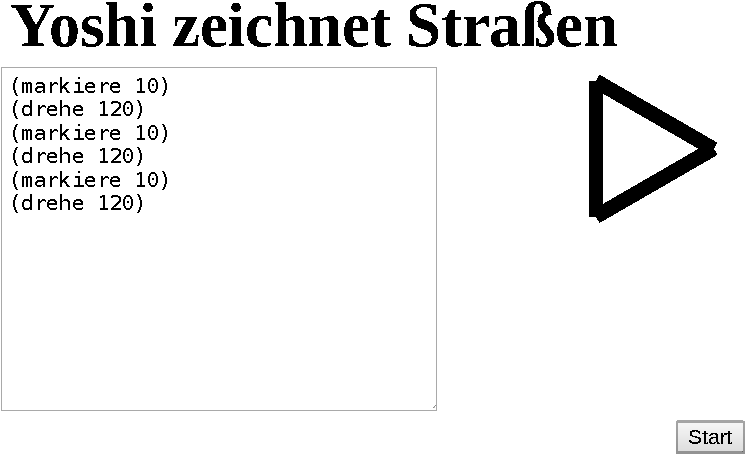
\includegraphics[scale=.8]{yoshi-3.pdf}}
\end{center}

\begin{multicols}{2}
	Nach Klick auf den „Start“-Knopf werden die Anweisungen ausgeführt.
	Das Ergebnis erscheint im anderen Feld.

	Sehen wir uns das Programm genauer an:

	\begin{Verbatim}
(markiere 10)
(drehe 120)
(markiere 10)
(drehe 120)
(markiere 10)
(drehe 120)
	\end{Verbatim}

	Jede Zeile ist eine eigene Anweisung.
	Jede Anweisung beginnt mit \verb|(| und endet mit
	\verb|)|.

	Die Anweisungen richten sich an eine unsichtbare Schildkröte, die
	in der Mitte des zweiten Feldes sitzt und nach oben sieht.

	Die erste Anweisung \verb|(markiere 10)| fordert die Schildkröte auf,
	10 Schritte in die aktuelle Richtung zu laufen.
	Dabei hinterläßt sie eine schwarze Linie.

	Die nächste Anweisung \verb|(drehe 120)| dreht die Schildkröte um
	$60$ Grad im Uhrzeigersinn. Sie blickt nun nach rechts/unten.
\end{multicols}
\end{document}
